% Paper 6 (T6) -- IEEE JBHI special issue "Integrating Imaging with Personalized Cardiovascular Medicine"
% Deadline 2026-10-15. Target: 8 pages (over-length charges start at page 9).
% Plan and word budgets: BENCHMARK-AND-PLAN-JBHI-2026-10-03.md
\documentclass[journal]{IEEEtran}
\usepackage{amsmath,amssymb}
\usepackage{graphicx}
\usepackage{booktabs}
\usepackage{siunitx}
\usepackage[hidelinks]{hyperref}

\begin{document}
\bstctlcite{IEEEexample:BSTcontrol}

\title{Topological Segmentation Error and Boundary-Condition Tuning in Computed Coronary FFR: A Controlled In
Silico Study}
% Working title; alternative from STUDY-PLAN-v2 sec. 0:
% "Matched at the Outlet, Wrong in the Tree: ..."

\author{Fadillah~Yamin,
        Mohd~Azan~Mohammed~Sapardi,
        Ming~Kwang~Tan,
        Xin~Wang,
        and~Mohd-Zulhilmi~Paiz~Ismadi%
\thanks{F. Yamin, X. Wang and M.-Z. P. Ismadi are with the Department of Mechanical Engineering, School of
Engineering, Monash University Malaysia, 47500 Bandar Sunway, Selangor, Malaysia (corresponding author:
M.-Z. P. Ismadi, e-mail: mohd.zulhilmi@monash.edu).}%
\thanks{M. A. Mohammed Sapardi is with the Department of Mechanical Engineering, Kulliyyah of Engineering,
International Islamic University Malaysia, 53100 Kuala Lumpur, Malaysia.}%
\thanks{M. K. Tan is with the Department of Mechanical Engineering, School of Engineering, Monash University
Malaysia, and the Department of Mechanical Engineering, Ming Chi University of Technology, New Taipei City 243,
Taiwan.}}

\markboth{IEEE Journal of Biomedical and Health Informatics}{Yamin \MakeLowercase{\textit{et al.}}: Segmentation Error and BC Tuning in Coronary FFR}

\maketitle

\begin{abstract}
Fractional flow reserve, the pressure ratio that decides whether a coronary narrowing is treated, can be computed
from computed tomography angiography. The computation depends on the segmented artery and on outlet boundary
conditions derived from it, often tuned to match measured perfusion. Whether tuning can hide a segmentation error
that changes the treatment decision at 0.80 has not been tested. We inserted stenoses into 150 coronary trees,
applied four segmentation error types (missed side branch, vessel break, longer lesion, narrowed taper), and
recomputed fractional flow reserve with a reduced-order model under three boundary-condition protocols: fixed,
re-derived from the corrupted tree, and tuned to the clean tree's territory perfusion, in two microvascular bed
structures. One case was solved in three dimensions. With fixed boundary conditions, the branching
(topological) errors changed the decision in 32--33\% of models, against 6--10\% for vessel-size (calibre) errors of inter-observer magnitude, close to the variability of repeat invasive measurement. Re-derived or tuned boundary
conditions reduced topological decision changes to 5--20\%. Tuning, however, removed the perfusion mismatch that
marked the error: 8--19\% of tuned models with a topological error passed a perfusion check stricter than
measurement repeatability while their fractional flow reserve was wrong by more than 0.05. In three dimensions,
prescribed territory flows reduced a missed-branch shift of 0.074 to below 0.001. A perfusion-matched coronary
model can thus pass validation with a material error in its fractional flow reserve. Detecting it requires a check
of the segmentation's branching structure and of the perfusion mismatch before tuning.
\end{abstract}

\begin{IEEEkeywords}
Boundary conditions, coronary artery disease, fractional flow reserve, image segmentation, reduced-order modeling,
uncertainty.
\end{IEEEkeywords}

% ---------------------------------------------------------------------------------------------------------------
\section{Introduction}
\IEEEPARstart{F}{ractional} flow reserve (FFR) is the pressure ratio that decides whether a coronary narrowing is
treated: the blood pressure beyond the narrowing divided by the aortic pressure during maximal flow. A value at or
below 0.80 marks a stenosis for revascularisation \cite{tonino2009}. FFR can also be computed without a pressure
wire. The lumen, the blood-filled channel of the artery, is segmented from coronary computed tomography (CT)
angiography and converted into a flow model, and the computed FFR has been validated against invasive measurement
in multicentre trials \cite{taylor2013,norgaard2014}. The calculation exists in three-dimensional (3D),
reduced-order and machine-learning forms \cite{kim2010,fossan2026,itu2016}. A reduced-order model replaces the 3D flow field
with a network of one-dimensional resistances.

Every such model needs boundary conditions: the pressures, flows or resistances imposed where the model ends, which
stand in for the vessels the image cannot resolve. The largest part of this unresolved circulation is the
microvascular bed, the arterioles and capillaries downstream of the segmented arteries, which set how much blood
each region of heart muscle draws. Its resistance is not measured but derived from the segmented lumen through
scaling laws that relate vessel size to the flow it carries \cite{murray1926,kim2010}. It is increasingly tuned so
that the model reproduces perfusion, the blood flow to each region of heart muscle, measured by imaging
\cite{menon2024}. The segmentation therefore enters the computed FFR twice: through the resistance of
the arteries it describes, and through the boundary conditions derived from them.

Segmentation error has been studied mainly as calibre error. Calibre is the inner diameter of a vessel, so a calibre error is a lumen drawn too wide or too narrow, or a narrowing drawn too long, while the branching is unchanged. Sensitivity analyses perturb the radius at fixed bifurcations and report a continuous change in the computed pressure index \cite{sankaran2015tmi,sankaran2015cmame,fernandez2024,dalmaso2025}. Studies that set geometry against
boundary conditions rank the two by their influence on a continuous output \cite{sankaran2016,tanade2022,korte2023}. Topological error, a change in the branching structure itself such as a missed side branch or a vessel that ends too early, has received less attention. In a one-dimensional model of the mouse pulmonary arteries, network connectivity contributed more to the uncertainty of the computed haemodynamics than vessel radius and length \cite{colebank2019}, and examples from a recent coronary benchmark showed vessel breaks in the output of every evaluated method despite high overlap scores \cite{bransby2026}. A missed branch removes part of the microvascular bed from the model and changes both the flow
through the stenosis and the boundary conditions derived from the tree.

Whether such an error reaches the computed FFR depends on how the boundary conditions are handled. With outlet resistance held fixed, adding a side branch beyond a stenosis lowered FFR by 15.5\% in an idealised model and by 13\% in one of two models built from optical coherence tomography \cite{gamage2022}. When a cohort-wide outlet resistance was recalibrated for a model with side-branch outflow, diagnostic accuracy changed little \cite{gosling2020}. In a clinical cohort, a change of outlet
model left the area under the receiver operating characteristic curve unchanged at 0.845 while sensitivity moved
from 58.1\% to 68.6\% \cite{fossan2026}. If the boundary conditions are tuned until the model matches measured
perfusion, a topological error may therefore disappear from the validation check while it remains in the pressure
along the vessel. None of these studies compares fixed, re-derived and tuned boundary conditions on the same
corrupted anatomy at the 0.80 threshold. Whether a model can pass a perfusion check and still assign the wrong
treatment class has not been tested.

We tested this with a controlled ablation, in which one error at a time is introduced into an otherwise correct
model. We inserted stenoses into 150 real coronary trees from a public CT angiography dataset so that the baseline
FFR spans the decision threshold, applied two topological and two calibre error types, and recomputed FFR with a
reduced-order model under fixed, re-derived and tuned boundary conditions in two microvascular bed structures. The
contributions are: (1) an error model that separates topological from calibre segmentation
error, with calibre magnitudes taken from measured inter-observer disagreement; (2) a paired comparison of the three
protocols at the 0.80 threshold against the variability of repeat invasive FFR, including the proportion of models
that pass a perfusion check while their FFR is materially wrong; and (3) a 3D computational fluid dynamics (CFD)
case study of the same mechanism on a segmented lumen.

% ---------------------------------------------------------------------------------------------------------------
\section{Methods}
\begin{figure*}[!t]\centering
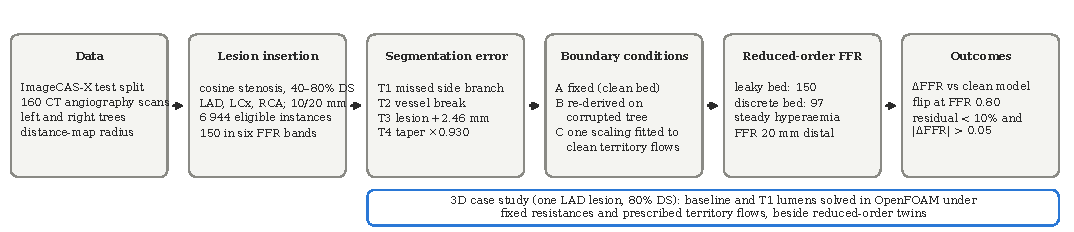
\includegraphics[width=\textwidth]{figures/fig1_design.pdf}
\caption{Study design. Each of 150 coronary instances is corrupted by four segmentation error types, solved under
three boundary-condition protocols in two bed structures, and compared with its own clean model. One
instance is also solved in three dimensions.}
\label{fig:design}
\end{figure*}
Fig.~\ref{fig:design} summarises the design. Every corrupted model is compared with its own clean model, so each
difference in FFR is caused by the error and the protocol alone.

\subsection{Data and Cohort}
ImageCAS-X provides voxel-wise lumen masks, labelled centrelines and surfaces for 800 CT angiography scans of the
ImageCAS dataset \cite{zeng2023,bransby2026,imagecasx_data}. We used its 160-scan test split, in which a second
analyst re-annotated each scan. The two annotators agreed to a Dice similarity coefficient (DSC, the overlap of two
masks) of 92.8\% and a 95th-percentile Hausdorff distance (HD95, the surface distance exceeded by 5\% of boundary
points) of 2.46~mm \cite{bransby2026}. Each scan gives a left and a right coronary tree. The radius at each centreline point is the distance from the point to the
lumen boundary in the mask, less half a voxel.

The dataset contains few lesions near the decision threshold, so we inserted one stenosis per instance into an
otherwise unchanged tree. An instance is one lesion in one tree. Five conditions made a host vessel (left anterior
descending, LAD; left circumflex, LCx; or right coronary artery, RCA) eligible. Image quality was graded at least adequate (2 on the dataset's scale of 0 to 4). The healthy reference radius $r_\mathrm{fit}$ at the lesion centre, from a linear taper
fit to the vessel, was at least 1.0~mm. Native narrowing between the lesion and the measurement point was below
40\% diameter stenosis (DS). The measurement point 20~mm beyond the lesion lay on a vessel of radius at least
0.75~mm. The FFR before insertion was at least 0.90. The lesion is an axisymmetric cosine narrowing,
\begin{equation}
\begin{aligned}
r'(s) &= \min\!\left(r,\; (1-w)\,r + w\,r_\mathrm{fit}\,(1-\mathrm{DS})\right),\\
w &= \tfrac{1}{2}\left[1+\cos\tfrac{2\pi (s-c)}{L}\right]
\end{aligned}
\end{equation}
for $|s-c|<L/2$, where $s$ is arc length, $c$ the lesion centre and $L$ its length. The vessel was never widened.
Lesions were centred 20 or 45~mm from the vessel origin, were 10 or 20~mm long and had 40, 50, 55, 60, 65, 70, 75
or 80\% DS. The full factorial gave 6\,944 instances on 280 host vessels from 140 scans. From these we drew 25
instances in each of six 0.05-wide bands of baseline FFR from 0.65 to 0.95, with at most two per tree. This gave
150 instances (50 per host vessel) in 108 trees from 93 patients.

\subsection{Reduced-Order FFR Model}
All 150 instances were solved with a reduced-order model, which represents the coronary tree as a network of flow
resistances instead of computing the full 3D flow field. The model places one node at every centreline point. Each element between consecutive nodes has the Poiseuille
resistance $8\mu\,\Delta s/(\pi r^4)$ of its actual radius $r$ and length $\Delta s$, with blood viscosity
$\mu = 0.004$~Pa\,s. Where the narrowing exceeds 30\% DS, an expansion loss $\Delta p = K\,Q|Q|$ is added at the
throat, with $K = \rho K_t (A_0/A_s - 1)^2 / (2A_0^2)$, $K_t = 1.52$ \cite{young1973}, density
$\rho = 1060$~kg\,m$^{-3}$, and $A_0$ and $A_s$ the reference and throat areas. Aortic pressure is 90~mmHg and
venous pressure 5~mmHg. Because the throat loss depends on flow, the equations are nonlinear and have no analytical solution
for a real tree. They are solved numerically by under-relaxed fixed-point iteration, each step a sparse linear
solve for the node pressures, until the relative flow change falls below $10^{-8}$. The mass-conservation error is recorded for every solve. FFR is the computed
pressure at the measurement point divided by aortic pressure. The model is steady and represents maximal hyperaemia
(maximal flow) without autoregulation.

The microvascular bed is modelled as conductances (the inverse of resistance) that drain flow from network nodes to
venous pressure. Each conductance depends on a healthy reference radius $r_\mathrm{ref}$, the taper-fit radius
$r_\mathrm{fit}$ made non-increasing along each path, and is scaled by one bed constant $C$. Two bed structures were analysed because they treat a deleted vessel differently. In the leaky
bed, flow leaves along the vessel wall at every node of the tree truncated at $r_\mathrm{ref} = 0.50$~mm, with
conductance $(r_\mathrm{ref}^3 - \sum r_{\mathrm{ref},\mathrm{child}}^3)/C$, so that flow follows Murray's cube law
\cite{murray1926}. This distributed outflow stands for the side branches the image does not resolve, and the
conductance of a deleted branch reappears as wall outflow at its parent node. In the discrete bed, flow leaves only
at the outlets of the tree truncated at $r_\mathrm{ref} = 0.60$~mm, with conductance $r_\mathrm{ref}^{2.66}/C$,
where the exponent approximates 8/3, the inverse of the 3/8 power that relates coronary vessel diameter to the
myocardial mass it perfuses \cite{choy2008}, so that outlet flow is taken as proportional to perfused mass. The discrete bed is the outlet structure that a 3D model can
represent. In both structures $C$ was calibrated on the healthy-equivalent network, the tree with its reference
radius and no lesion, so that inflow equals the hyperaemic demand $Q = k\,r_\mathrm{in}^3$, where $r_\mathrm{in}$ is
the inlet radius and the cube law is Murray's \cite{murray1926}. With the model setting $k = 562$~s$^{-1}$, a
vessel with the normal proximal LAD diameter of 3.7~mm \cite{dodge1992}, carries 214~mL/min,
within one standard deviation of the hyperaemic flow measured in that artery by continuous thermodilution
($228 \pm 71$ to $293 \pm 102$~mL/min) \cite{fournier2021}. For the median inlet radius of this cohort, 1.39~mm, the
demand was 1.5~mL/s. Reference radii and $C$ are computed from the original tree, so an inserted lesion changes
only the epicardial radius. The leaky bed was analysed on all 150 instances. The discrete bed was analysed on the
97 instances whose healthy-equivalent network gave a main-vessel FFR of at least 0.90 and had at least two outlets,
and baseline FFR bands were derived separately for each bed. Halving the centreline spacing changed FFR by at most
0.005 in either bed.

\subsection{Segmentation Error Types}
\begin{table}[!t]
\caption{Segmentation Error Types and Boundary-Condition Protocols}
\label{tab:design}
\centering\footnotesize
\begin{tabular}{@{}p{0.6cm}p{4.9cm}p{2.5cm}@{}}
\toprule
 & Definition & Magnitude (source)\\
\midrule
T1 & Missed branch: largest side branch distal to the lesion deleted with its subtree (topological) & Largest eligible branch (design)\\
T2 & Vessel break: host vessel ended beyond the measurement point (topological) & 25~mm past lesion edge (design)\\
T3 & Lesion length over-estimated (calibre) & $+2.46$~mm (inter-observer HD95)\\
T4 & Taper: lumen under-sized from the lesion distally (calibre) & Radius $\times 0.930$ (inter-observer DSC)\\
\midrule
A & Fixed: surviving nodes keep the clean bed conductances and $C$ & --\\
B & Re-derived: bed rule and $C$ recomputed on the corrupted tree & --\\
C & Tuned: one scaling of $C$ fitted to the clean territory flows & One parameter, $\geq 2$ targets\\
\bottomrule
\end{tabular}
\end{table}
Four error types were applied to each instance with its lesion in place (Table~\ref{tab:design}). Two are
topological errors, which change which vessels exist. Two are calibre errors, which change the lumen size or lesion
extent while the branching is unchanged. The missed branch (T1) deletes the largest side branch that leaves the host
vessel beyond the lesion, together with its subtree. The vessel break (T2) ends the host vessel 25~mm beyond the
distal edge of the lesion, so the measurement point survives but the run-off beyond it is lost. The lesion length
(T3) re-inserts the same stenosis 2.46~mm longer. The taper (T4) multiplies the radius by 0.930 from the proximal
edge of the lesion onwards and in every descendant vessel. For T3 and T4 the set of modelled nodes is fixed to that
of the clean tree, so a narrowed radius does not remove an outlet.

The calibre magnitudes are the inter-observer statistics of the test split, so each calibre error is as large as
the disagreement between two annotators. HD95 (2.46~mm) sets T3. The DSC of 92.8\% sets T4 as the radius
ratio $k$ of two coaxial cylinders, $2k^2/(k^2+1) = 0.928$. Because both annotators edited the same automatically
generated centrelines, the dataset authors describe the inter-observer DSC as an upper bound on agreement \cite{bransby2026}. T1 and T2 have
no measured magnitude and are design choices. Nodes of the corrupted tree were matched to the clean tree by
coordinate, and FFR was read at the same anatomical point.

\subsection{Boundary-Condition Protocols}
Each corrupted tree was solved under three protocols (Table~\ref{tab:design}). Under Protocol A (fixed), surviving
nodes keep the bed conductances and $C$ of the clean model, and the bed of deleted vessels is lost. This represents
the case in which the boundary conditions were obtained correctly despite the segmentation error. Under Protocol B
(re-derived), the bed rule is applied to the corrupted tree and $C$ is recalibrated to that tree's own hyperaemic
demand, as an automated pipeline does with whatever anatomy it receives. Under Protocol C (tuned), one global
scaling of $C$ (one bed scaling) is fitted so that the corrupted model reproduces the clean model's territory
flows. A perfusion territory is the subtree below each child of
the first bifurcation of the clean tree. Its target is the total bed outflow of that subtree in the clean model,
including the share of any vessel the error deleted, because the heart muscle is perfused whether or not its artery
was segmented. Each corrupted node belongs to the territory of its clean counterpart. The fit minimised the mean
squared relative error of the territory flows over a 61-point grid spanning $\pm 1.5$ decades of $C$ about the
re-derived value, followed by bounded refinement. A fit at the edge of the search range was recorded as a failure.
One parameter against two or more targets makes the fit over-determined, so this is the least flexible tuning a
pipeline could use. Protocol C is therefore defined only when at least two territories retain a vessel. It matches
flow only, because matching both flow and pressure at the outlets of a steady tree would reproduce the clean FFR by
construction.

For every protocol we computed the perfusion residual, the root mean square of the relative differences between the
model's territory flows and the clean targets. It is the quantity a perfusion check compares with the measurement.

\subsection{Three-Dimensional Case Study}
To test whether the findings depend on the simplifications of the reduced-order model, one instance (a 20~mm lesion
of 80\% DS in the proximal LAD) was also solved with 3D CFD, which computes the full velocity and pressure fields
from the Navier--Stokes equations. These have no analytical solution for a real artery, so they were solved
numerically by the finite-volume method. Three lumens were built: clean, with the lesion (baseline), and with the
lesion and the missed branch (T1). Surfaces were extracted from the mask by marching cubes and Taubin smoothing; the
lesion was applied by moving surface vertices radially with (1), and the branch was removed by deleting its voxels.
Meshes of 3.5--3.9 million cells (cfMesh) had 25~\textmu m cells within $\pm 4$~mm of the throat and four boundary
layers.

Steady laminar Newtonian flow, with the viscosity and density of the reduced-order model, was solved with the
steady incompressible solver of OpenFOAM (simpleFoam, ESI v2406, SIMPLE pressure--velocity coupling), with a
bounded second-order upwind scheme for convection and second-order central schemes elsewhere. Each solve ran
3\,000 iterations; convergence required scaled residuals below $10^{-5}$ and a steady pressure at the measurement
point. The walls were rigid with no slip, and the inlet carried aortic pressure. Each outlet either set its pressure
to venous pressure plus the clean tree's resistance times its flow (Protocol A), or received a prescribed clean
territory flow, shared over the territory's surviving outlets by bed weight (the per-outlet form of Protocol C). FFR
is the area-averaged pressure on a cross-section at the measurement point divided by aortic pressure. A
grid-convergence study on an idealised 70\% DS stenosis (throat cells of 50, 25 and 12.5~\textmu m) gave a
discretisation uncertainty in FFR of $5.5\times10^{-4}$. A reduced-order twin of each geometry, rebuilt on the
area-equivalent radius of the meshed lumen with the same outlet conditions, separates the effect of model fidelity
from that of radius definition.

\subsection{Outcomes and Statistical Analysis}
For each instance, error type, protocol and bed, $\Delta$FFR is the corrupted model's FFR minus that of the
instance's own clean model in the same bed. A flip is a change of classification at 0.80 between the two, that is,
a change in the treatment decision. A model passes the perfusion check when its perfusion residual is below 10\%.
Published repeatability of hyperaemic myocardial blood flow (within-subject variation of 10--15\% \cite{schindler2023}; regional repeatability coefficient of 30--37\% \cite{brown2018}) implies a 95\% bound of about 20--29\% for a comparison of one deterministic model output with one regional measurement. The 10\% threshold is therefore strict, and a looser
threshold can only increase the number of models that pass. Thresholds of 13\% and 16\% were analysed as
sensitivities. An FFR is materially wrong when $|\Delta\mathrm{FFR}| > 0.05$, an error large enough to matter near
the 0.80 cut.

Proportions are reported with Wilson 95\% confidence intervals (CIs). Protocol contrasts (B against A, C against A,
C against B) are paired within instance and tested with the exact McNemar test, with Holm adjustment across the
three contrasts of each error type and bed. Topological and calibre errors are compared by a paired sign test on
the per-instance flip proportions of each class, and paired changes in $|\Delta\mathrm{FFR}|$ by the Wilcoxon
signed-rank test. Flips were also modelled by a Bayesian mixed-effects logistic regression fitted by variational
inference, with error type, protocol and their interaction, severity, length and baseline band as fixed effects and
random intercepts for patient and lesion slot (Supplementary Material). Because the two beds differ in structure,
every analysis was run in both, effect sizes are reported per bed, and a finding is claimed only where its
direction agrees in both.

Each flip rate is compared with a noise floor, the rate expected from measurement variability alone. For each instance, this is the probability that a repeat invasive FFR, drawn from a normal
distribution centred on the clean value with the published standard deviation of the difference between repeat measurements, 0.018 \cite{johnson2015}, falls on the other side of 0.80, following the measurement-certainty approach of \cite{petraco2013}. A second floor was simulated on the clean anatomy: 20 draws
per instance perturbed cardiac output, aortic pressure, blood viscosity, the share of flow to each territory and the
measured territory flows by their within-subject variability, and the model was tuned to the perturbed flows as in
Protocol C.

The cohort, design, analysis plan and ablation code were fixed, and the cohort list hashed, before the ablation was
run. The analysis script was written while the ablation ran and before its output was read. Departures from the
plan are listed in the Supplementary Material.

% ---------------------------------------------------------------------------------------------------------------
\section{Results}
% Source: results/ablation-2026-10-07.csv -> code/analyse_ablation.py -> results/analysis-ablation-2026-10-07/;
% Table II rows from code/table2.py; Figs. 2-4 from code/fig_results.py.
\subsection{Decision Changes by Error Type and Protocol}
All 2\,599 corrupted-model solves converged (maximum mass-conservation error $9\times10^{-9}$). A missed branch
was possible in 77 of 97 instances in the discrete bed and 118
of 150 in the leaky bed, and a vessel break in 96 and 149. Protocol C was undefined for 33 and 47 of the
missed-branch instances and for 36 and 49 of the vessel breaks, all but four in the RCA. In the discrete bed, the
vessel break removed every outlet in 36 instances under Protocol A.

\begin{table*}[!t]
\caption{Decision Changes and Absorption by Error Type, Protocol and Bed Structure}
\label{tab:results}
\centering\footnotesize
\begin{tabular}{@{}llrccrcc@{}}
\toprule
 & & \multicolumn{3}{c}{Discrete bed (97 instances)} & \multicolumn{3}{c}{Leaky bed (150 instances)}\\
\cmidrule(lr){3-5}\cmidrule(l){6-8}
Error & Protocol & $n$ & Flip, \% & Passes and wrong, \% & $n$ & Flip, \% & Passes and wrong, \%\\
\midrule
T1 & A & 77 & 27 (19--38) & 13 (7--22) & 118 & 18 (12--26) & 16 (11--24) \\
 & B & 77 & 9 (4--18) & 1 (0--7) & 118 & 5 (2--11) & 5 (2--11) \\
 & C & 44 & 18 (10--32) & 20 (11--35) & 71 & 8 (4--17) & 11 (6--21) \\
\addlinespace[2pt]
T2 & A & 60 & 40 (29--53) & 12 (6--22) & 147 & 43 (35--51) & 24 (17--33) \\
 & B & 96 & 18 (11--27) & 2 (0--9) & 149 & 5 (2--9) & 4 (2--10) \\
 & C & 60 & 20 (12--32) & 18 (11--30) & 100 & 8 (4--15) & 6 (3--12) \\
\addlinespace[2pt]
T3 & A & 97 & 7 (4--14) & 0 (0--4) & 150 & 2 (1--6) & 0 (0--2) \\
 & B & 97 & 7 (4--14) & 0 (0--4) & 150 & 2 (1--6) & 0 (0--2) \\
 & C & 97 & 7 (4--14) & 0 (0--4) & 150 & 3 (1--7) & 1 (0--4) \\
\addlinespace[2pt]
T4 & A & 97 & 13 (8--22) & 6 (3--13) & 150 & 9 (6--15) & 7 (4--12) \\
 & B & 97 & 8 (4--15) & 0 (0--4) & 150 & 1 (0--4) & 0 (0--2) \\
 & C & 97 & 8 (4--15) & 9 (5--17) & 150 & 5 (3--10) & 24 (18--31) \\
\bottomrule
\end{tabular}
\\[2pt]
\parbox{\textwidth}{\footnotesize Flip: change of classification at FFR 0.80. Passes and wrong: territory-perfusion
residual below 10\% and $|\Delta\mathrm{FFR}| > 0.05$, over models with a defined residual (T2 under B in the discrete
bed, $n = 60$; T2 under A and B in the leaky bed, $n = 100$). Wilson 95\% intervals in parentheses. The expected flip
rate from repeat invasive measurement is 5.0--6.5\% across cells.}
\end{table*}

Topological errors changed the decision more often than calibre errors under every protocol and in both beds
(Table~\ref{tab:results}). With fixed boundary conditions in the discrete bed, 45 of 137 topological-error models
(33\%, 95\% CI 26--41\%) crossed 0.80, against 20 of 194 calibre-error models (10\%, 7--15\%). In the leaky bed the
proportions were 32\% (26--38\%) and 6\% (4--9\%) (paired sign test, $p \leq 0.002$ in both beds). Under
Protocols B and C the difference kept its direction. It was significant in the discrete bed
($p = 0.013$ and 0.002) but not in the leaky bed ($p = 0.18$ and 0.057). Flips were concentrated in the bands
adjacent to 0.80 (Fig.~\ref{fig:band}).

The calibre errors rarely changed the decision. At the magnitude of inter-observer disagreement they changed FFR by
a mean of 0.006--0.037 in absolute value, and their flip rates of 1--13\% were of the order of the 5.0--6.5\%
expected from repeat invasive measurement. Only the taper under fixed boundary conditions exceeded this noise floor
with its lower confidence bound, at 13\% in the discrete bed and 9\% in the leaky bed (Table~\ref{tab:results}).

Re-deriving the boundary conditions from the corrupted tree (Protocol B) produced the fewest flips. Against
Protocol A, it reversed 14 of 21 missed-branch flips in the discrete bed and 15 of 21 in the leaky bed, and created
none (McNemar, Holm-adjusted $p < 0.001$ for both). It reversed 56 of 63 vessel-break flips in the leaky bed
($p < 0.001$). In the discrete bed it reversed 22 vessel-break flips but created 12 ($p = 0.24$), because the
re-derived bed lowered FFR below the clean value (mean $\Delta$FFR $-0.039$). Protocol B models, however, failed
their own perfusion check most often.

\begin{figure*}[!t]\centering
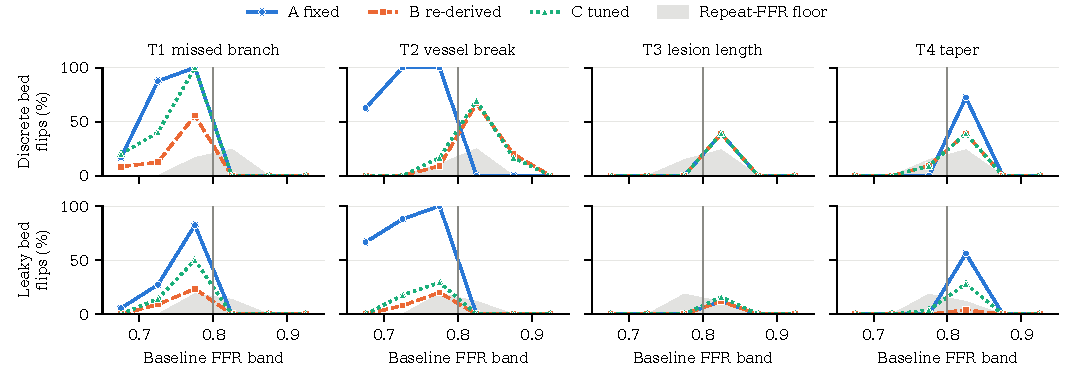
\includegraphics[width=\textwidth]{figures/fig2_flip_by_band.pdf}
\caption{Flip rate (proportion of models whose classification at FFR 0.80 changed) by baseline FFR band (0.05
wide, plotted at the band centre; bands with fewer than three models omitted), error type, protocol and bed
structure. Shaded: flip rate expected from repeat invasive FFR alone (standard deviation 0.018).}
\label{fig:band}
\end{figure*}

\subsection{Absorption Under Tuned Boundary Conditions}
We call it absorption when tuning removes the error from the perfusion check but not from the FFR. Fitting one bed
scaling to the clean territory flows (Protocol C) lowered the median perfusion residual of topological-error models
from 0.19 to 0.14 in the discrete bed and from 0.10 to 0.02 in the leaky bed. Compared with Protocol A, tuning
reversed 4 missed-branch flips and created none in each bed ($p = 0.25$). For vessel breaks it reversed 32 flips
and created none in the leaky bed ($p < 0.001$), and reversed 22 and created 10 in the discrete bed ($p = 0.15$).
We had expected tuning to leave the flip rate at or above that of fixed boundary conditions. Instead, where the
change was resolved, it was a reduction. Relative to re-derived boundary conditions (Protocol B), tuning changed at
most two topological-error decisions per cell ($p \geq 0.5$), while it lowered the median residual of missed-branch
models from 0.36 to 0.16 (discrete) and from 0.04 to 0.03 (leaky).

Tuning did not remove the error from the FFR (Fig.~\ref{fig:absorb}). Of the tuned topological-error models, 20 of
104 (19\%, 13--28\%) in the discrete bed and 14 of 171 (8\%, 5--13\%) in the leaky bed passed the perfusion check
while their FFR was materially wrong (more than 0.05 from the clean value). In the discrete bed these were half of
the 39 models that passed. Four and 12 of the passing models, respectively, also changed the decision. Models with
correct anatomy, tuned to perfusion measured with physiological noise, passed while materially wrong in 3.1\% (2.4--4.0\%) and 3.9\% (3.2--4.6\%) of draws, and their flip rates were 6.2\% and 7.2\%.
The proportion depended on the assumed hyperaemic demand. With the demand scaled by 0.7 and 1.3, it was 12\% and
25\% in the discrete bed and 3\% and 12\% in the leaky bed, but the ordering of topological against calibre errors
and of Protocols B and C against A was unchanged (Supplementary Material). Under Protocol A the same proportions
were 12\% and 20\%; the ordering of A and C differed between the beds, so no difference between them is claimed. At
the looser validation thresholds of 13\% and 16\%, the proportion under Protocol C rose to 28\% (20--37\%) and 38\%
(30--48\%) in the discrete bed and was 9\% (6--15\%) at both in the leaky bed.

Tuning also enlarged the taper error: in the leaky bed, 36 of 150 tuned taper models (24\%, 18--31\%) passed while
materially wrong, against 10 under Protocol A (Table~\ref{tab:results}).

\begin{figure}[!t]\centering
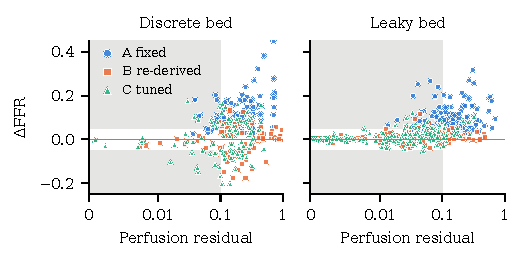
\includegraphics[width=\columnwidth]{figures/fig3_absorption.pdf}
\caption{Change in FFR against territory-perfusion residual for missed-branch and vessel-break models. Each point
is one model. Shaded: models that pass the perfusion check (residual $< 0.10$) while materially wrong
($|\Delta\mathrm{FFR}| > 0.05$). Horizontal axis linear below 0.01 and logarithmic above.}
\label{fig:absorb}
\end{figure}

\subsection{Side-Branch Loss Under Fixed and Tuned Resistance}
A missed side branch raised the computed FFR, and tuning removed only part of the rise. In the 44 (discrete) and 71
(leaky) instances in which Protocol C was defined, the missed branch raised FFR by a median of 0.095 and 0.047 with
fixed boundary conditions. The shift exceeded 13\% of the clean FFR in 45\% and 11\% of these instances. Tuning
reduced the shift to a median of 0.077 and 0.015 (Wilcoxon signed-rank, $p < 0.001$ in both beds;
Fig.~\ref{fig:branch}). In the leaky bed the tuned shift was a median 42\% of the fixed shift, and 12 of 71 instances
remained above 0.05. In the discrete bed it was 84\%, and 33 of 44 remained above 0.05.

\begin{figure}[!t]\centering
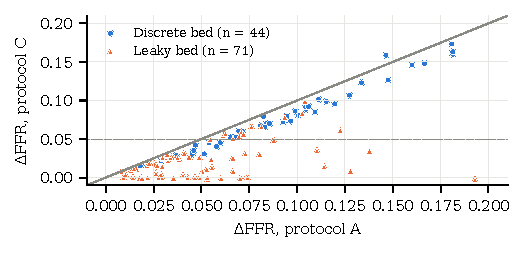
\includegraphics[width=\columnwidth]{figures/fig4_branch_loss.pdf}
\caption{Change in FFR caused by a missed side branch under fixed boundary conditions (Protocol A) and after tuning
to territory flows (Protocol C), paired by instance. Solid line: identity. Dashed line: $\Delta$FFR $= 0.05$.}
\label{fig:branch}
\end{figure}

\subsection{Three-Dimensional Case Study}
The 3D solution showed the same concealment. With the clean tree's resistances at the outlets, removal of the side
branch raised the 3D FFR at the measurement point from 0.870 to 0.944 ($\Delta$FFR $= +0.074$). With the clean
territory flows prescribed at the outlets, the same error changed FFR by $-0.0007$ (0.892 in both geometries). The
reduced-order twins gave $+0.081$ and $-0.0005$ for the same two conditions, and their baseline FFR was within 0.011
of the 3D values (Fig.~\ref{fig:case3d}).
\begin{figure*}[!t]\centering
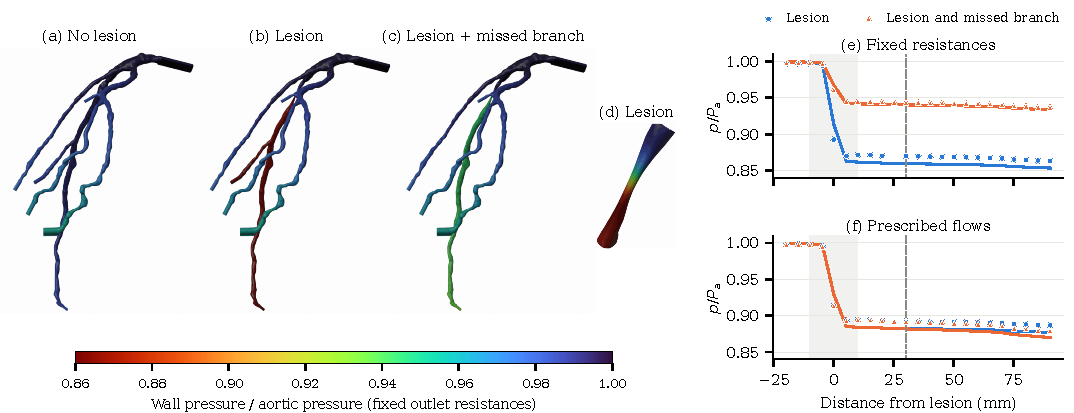
\includegraphics[width=\textwidth]{figures/fig5_case3d.pdf}
\caption{Three-dimensional case study (proximal LAD, 80\% DS). (a)--(c) Wall pressure relative to aortic pressure
with the clean tree's outlet resistances: without the lesion, with the lesion, and with the lesion and a missed
side branch. The lesion lowers the downstream pressure (red); the missed branch raises it again (green), a shift
that would move a decision near 0.80. (d) Close-up of the lesion. (e), (f) Pressure along the artery with fixed
resistances and with prescribed clean territory flows. Markers: 3D cross-section averages. Lines: reduced-order
models on the meshed radius with the same outlet conditions. Shaded: lesion. Dashed: measurement point.}
\label{fig:case3d}
\end{figure*} Two caveats apply. The meshed lumen was wider than the radius used by the reduced-order model (median
difference 0.14~mm; throat area-equivalent radius 0.276 against 0.231~mm), and on the requested radius the
reduced-order baseline was 0.761. Halving the cell size in the throat zone to 12.5~\textmu m changed the baseline
FFR by 0.0019 and 0.0021 in two zone placements, against the error effect of 0.074, and a regenerated mesh at
25~\textmu m reproduced the baseline value.

% ---------------------------------------------------------------------------------------------------------------
\section{Discussion}
\subsection{Concealment at Calibration}
This study asked whether tuning a coronary flow model to perfusion can hide a segmentation error that changes the
treatment decision. Three findings answer it. First, the decision risk of segmentation lies mainly in the branching structure of the lumen, not in its calibre.
With fixed boundary conditions, a topological error (a missed branch or a vessel break) changed the decision at
0.80 three to six times as often as a calibre error of inter-observer magnitude. The calibre errors produced flip
rates of the order of repeat invasive measurement.

Second, how much of a topological error reaches the decision depends on the boundary conditions. With the clean bed
held fixed, a missed branch or a vessel break flipped 18--43\% of decisions. Re-deriving the bed from the corrupted
tree reduced this to 5--18\%, and tuning one bed scaling to territory flows gave 8--20\%. We had expected tuning to
leave the flip rate at or above that of fixed boundary conditions. Instead it moved the decision towards the clean
result.

Third, tuning separated the validation check from the error. Re-derived models carried the error in their perfusion
residual (median 0.36 for a missed branch in the discrete bed), so a perfusion check flagged them. Tuning lowered
that residual to 0.16 without changing more than two decisions per cell. In the discrete bed, half of the tuned
topological-error models that passed the check had an FFR error larger than 0.05. The check therefore measured
agreement with the targets that were fitted, not the correctness of the model. The remaining error sat in the
pressure distribution along the vessel, which one global scaling cannot restore once a branch is absent. The three-dimensional case showed the same mechanism.

Bed structure set the magnitude of these effects. In the leaky bed, the conductance of a deleted branch reappears
as wall outflow at its parent node, which damps the missed-branch error before any tuning. The discrete bed, which
corresponds to the outlet structure of a three-dimensional model, retained 84\% of the missed-branch shift after
tuning. Claims are therefore restricted to directions that held in both structures.

\subsection{Relation to Published Studies}
Published sensitivity analyses of computed pressure indices perturb lumen calibre with the branching structure fixed and report
continuous sensitivity \cite{sankaran2015tmi,sankaran2015cmame,fernandez2024,dalmaso2025}. Our calibre errors fall within that framework and rarely changed the decision. Studies that compare geometry with boundary conditions rank their influence on a continuous output
\cite{sankaran2016,tanade2022,korte2023}. The present results add that the ranking depends on the error type and on
the boundary-condition protocol, and that the decision outcome separates them more clearly than the continuous
one.

Two earlier findings that appeared to disagree are reproduced here. A side-branch effect of 13--15.5\% under fixed outlet resistance was reported in an idealised model and a model built from optical coherence tomography \cite{gamage2022}, whereas recalibrating a cohort-wide outlet resistance absorbed a large change in side-branch flow with little change in diagnostic accuracy \cite{gosling2020}. In our cohort, the missed-branch shift exceeded 13\% of the clean FFR in 45\%
(discrete) and 11\% (leaky) of instances with fixed resistance, and tuning reduced it. The difference between the
two findings therefore follows from the boundary-condition protocol. A change of
the outlet model in a clinical computed-FFR cohort left the area under the curve unchanged while sensitivity
changed \cite{fossan2026}. The protocol effect observed here, 43\% against 5\% of decisions changed by a vessel break on identical anatomy (leaky bed), is consistent with that observation.

Vessel breaks occur in the output of current coronary segmentation methods despite high overlap scores \cite{bransby2026}, and a missing side branch removes few voxels from the tree, so overlap changes little when it is absent. The error types that carried the decision risk
in this study are therefore the ones that the usual segmentation metrics do not measure.

\subsection{Implications for Model Validation}
Perfusion imaging is used to personalise coronary flow models \cite{menon2024}. In this study, passing a
perfusion check stricter than the repeatability of the measurement did not establish that the FFR was correct:
8--19\% of tuned topological-error models passed with a material FFR error. The perfusion residual before tuning
was informative, because re-derived models carried a large residual when a branch was missing. Two additions to
current reporting would expose the errors that the tuned residual conceals: the untuned residual beside the tuned
one, and the topological agreement of the segmentation (branch completeness and connectivity) beside its overlap
score.

\subsection{Limitations}
The stenoses were inserted into healthy vessels to obtain lesions near the threshold, so the lesion geometry is
idealised. The reduced-order model is steady, without autoregulation or heart-rate effects. The magnitudes of the
missed-branch and vessel-break errors are design choices, and the calibre magnitudes come from inter-observer
statistics that are likely to overstate agreement. Protocol C used one global scaling, the least flexible tuning, and
a per-territory scaling was not evaluated. Protocol C was undefined for most right coronary instances with a
topological error, so the tuned-protocol results for these error types describe the left coronary tree. The
three-dimensional analysis covers one instance, and its meshed lumen was wider than the radius used by the
reduced-order model. No invasive FFR was available, so the noise floor was modelled from published repeat
measurements.

\section{Conclusion}
In 150 coronary trees with controlled stenoses and fixed boundary conditions, topological segmentation errors
changed the decision at FFR 0.80 three to six times as often as calibre errors of inter-observer magnitude, which
were close to the repeatability of invasive measurement. The boundary-condition protocol alone changed how often a topological error altered the decision. For a vessel break in the leaky bed, the proportion fell from 43\% of models with fixed boundary conditions to 5\% with re-derived ones. Tuning one bed scaling to territory flows reduced decision changes
but removed the perfusion residual that marked the error, and 8--19\% of tuned models passed a perfusion check while
their FFR was wrong by more than 0.05. A three-dimensional case reproduced the concealment of a missed side branch
under prescribed flows.

\section*{Data and Code Availability}
ImageCAS-X is available under CC BY 4.0 (doi:10.5281/zenodo.21887809). The code and the frozen cohort list are
available from the corresponding author on request.

\section*{Conflict of Interest}
The authors declare no conflicts of interest.

\section*{Acknowledgment}
This work received no external funding. The study used a public, anonymised dataset and required no ethics
approval.

\bibliographystyle{IEEEtran}
\bibliography{refs}

\end{document}
